\section{MDPS}
\label{sec:mdps}

\subsection{Markov chains}

Markov Chains consists of states and their transition probabilities.

\begin{figure}[h]
    \centering
        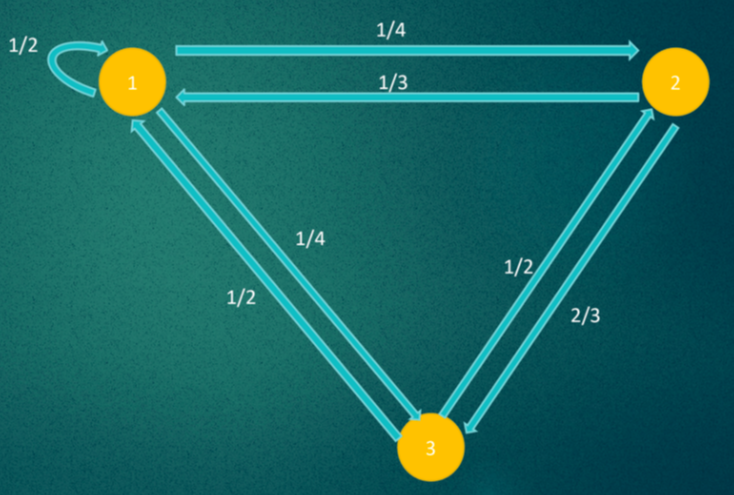
\includegraphics[width=0.8\textwidth]{figures/MDPS/chain.png}\\
        \caption{Markov Chain}
\end{figure}

\subsection{Markov Decision Processes}

A Markov Decision Process is a Markov Chain, in addition to actions and rewards.

\begin{figure}[h]
    \centering
        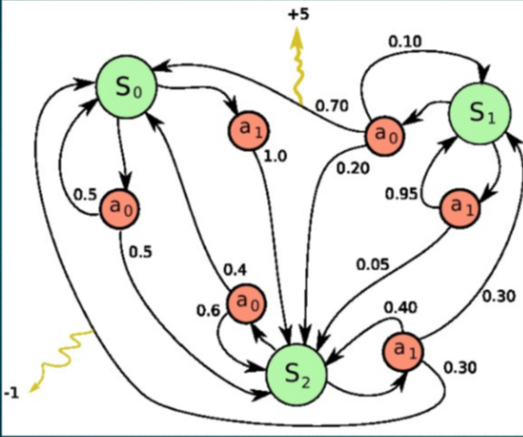
\includegraphics[width=0.5\textwidth]{figures/MDPS/mdp.png}\\
        \caption{MDP Illustrated}
\end{figure}

A markov decision process contains
\begin{itemize}
    \item States
    \item Actions
    \item Transition fucntion
    \item Reward
\end{itemize}



\subsubsection{States}

A MDP state is a unique characterization of all important information in a state of the problem that is modeled. The state space $S$ is the set of environmental states ${s_1, s_2, ..., s_n}$ $\in$ $S$.

\subsubsection{Actions}

The set of actions is the finite set ${a_1, a_2, ..., a_n}$ $\in$ $S$. The action space is restricted by the environmental state and becomes $A(s)$ $\subseteq $ $A$.

\subsubsection{Transition function}

The transition function $T$ is defined as $T: S x A x S -> [0, 1]$. I. e. the transition function takes in a current state, a possible action, and returns the probability of the next state. It is also denoted $T(s, a, s')$.
The transition function adheres to the Markov assumption, that is, the current state s gives enough information to make an optimal decision. Previous states are of no significance.

\subsubsection{Reward function}

The reward function $R: S x A x S -> \mathcal{R}$ takes in a current state, an action from the current state and a possible next state and returns a scalar value. It gives the reward of going from one state to another based on the performed action.


\subsubsection{MDP definition}

A MDP is a tuple $\bigl< S, A, T, R \bigr>$. The transition function $T$ and the reward function $R$ together define the model of the MDP. 

The MDP process becomes a state-action-reward history $(s_0, a_0, r_0), ..., (s_n, a_n, r_n)$.
Episodic tasks is a task of some episodic length, where the goal is to take the agent from a  starting state to a goal state. If a task is episodic, we obtain a state-action-reward history $(s_0, a_0, r_0), ..., (s_{goal}, a_{goal}, r_{goal} $ where the process ends in state $s_{goal}$ and then starts again. 


MDPs can be model based or model free:
\begin{itemize}
    \item \textbf{Model based}: Full transition dynamics and reward distribution is known. This kind of problem can be solved using dynamic programming.
    \item \textbf{Model free}: When there is no model of the environment and the agent has to explore to get familiar with it and optimize its policy.
\end{itemize}


\subsubsection{Policies}

Given an MDP $\bigl< S, A, T, R \bigr>$, the policy $\pi$ is a function $\pi:$ $S$ -> $A$, i. e, it maps the state to an action. 


\subsubsection{Optimality criteria}

\begin{itemize}
    \item With a finite horizon, the agent usually is set to optimize the expected reward over the specified time horizon,  $E \bigl[ \sum_{t=0}^{h} r_t \bigr]$.
    \item With an infinite horizon, the agent is set up to optimize a discounted expected reward, which makes it prioritize rewards in the near future more than distant rewards,
    $E \bigl[ \sum_{t=0}^{\infty} \gamma^t r_t \bigr]$. This also leads to better convergence properties and formal convergence proofs.
    \item One can also optimize for the average reward over a finite horizon,
    $ \lim_{h-> \infty} E \bigl[ \frac{1}{h} \sum_{t=0}^{h} r_t \bigr]$
\end{itemize}

\subsubsection{Value functions and Bellman equations}

The value function is a measure of the value of being in state $s$, and following policy $\pi$ thereafter. The state-value function is a measure of the value of being in state $s$, taking action $a$, and following the policy $\pi$ thereafter. The values returned is the expected sum of rewards. Both functions link optimality criteria to policies, and most learning algorithms for MDPs compute optimal policies by learning value functions.

Greedy policy: Optimal action given the optimal state-value function $V^*$:

\begin{align}
    \pi^*(s) = \text{argmax}_a \sum_{s'} T(s, a, s')(R(s, a, s') + \gamma V^*(s'))
\end{align}

The relation between the state-value function $V^{\pi}(s)$ and the action-value function
$Q^{\pi}(s, a)$ is 

\begin{align}
    V^*(s) = \text{max}_a Q^{\pi}(s, a)
\end{align}

Again, the optimal policy can be described as

\begin{align}
    \pi^*(s) = \text{argmax}_a Q^{*}(s, a)
\end{align}

The state-value function does \textit{not} evaluate the possible actions,
and thus it cannot be optimized in the same manner as the action-value function. In model free approaches where T and R are unknown, Q-functions are learned instead of V-functions. This is due to the fact that we are uncertain about our policy, and it thus makes sense to compare the value of possible actions up against the value of the action chosen by the policy.

\subsubsection{Exploration vs exploitation}

Studies have shown that always choosing the optimal action (greedy policy) has worse convergence properties than when including a probability $\epsilon$ of taking some other action. This makes the agent explore and discover more aspects of the environment than it would have by choosing the optimal action. 





